
%% bare_conf.tex
%% V1.3
%% 2007/01/11
%% by Michael Shell
%% See:
%% http://www.michaelshell.org/
%% for current contact information.
%%
%% This is a skeleton file demonstrating the use of IEEEtran.cls
%% (requires IEEEtran.cls version 1.7 or later) with an IEEE conference paper.
%%
%% Support sites:
%% http://www.michaelshell.org/tex/ieeetran/
%% http://www.ctan.org/tex-archive/macros/latex/contrib/IEEEtran/
%% and
%% http://www.ieee.org/

%%*************************************************************************
%% Legal Notice:
%% This code is offered as-is without any warranty either expressed or
%% implied; without even the implied warranty of MERCHANTABILITY or
%% FITNESS FOR A PARTICULAR PURPOSE! 
%% User assumes all risk.
%% In no event shall IEEE or any contributor to this code be liable for
%% any damages or losses, including, but not limited to, incidental,
%% consequential, or any other damages, resulting from the use or misuse
%% of any information contained here.
%%
%% All comments are the opinions of their respective authors and are not
%% necessarily endorsed by the IEEE.
%%
%% This work is distributed under the LaTeX Project Public License (LPPL)
%% ( http://www.latex-project.org/ ) version 1.3, and may be freely used,
%% distributed and modified. A copy of the LPPL, version 1.3, is included
%% in the base LaTeX documentation of all distributions of LaTeX released
%% 2003/12/01 or later.
%% Retain all contribution notices and credits.
%% ** Modified files should be clearly indicated as such, including  **
%% ** renaming them and changing author support contact information. **
%%
%% File list of work: IEEEtran.cls, IEEEtran_HOWTO.pdf, bare_adv.tex,
%%                    bare_conf.tex, bare_jrnl.tex, bare_jrnl_compsoc.tex
%%*************************************************************************

% *** Authors should verify (and, if needed, correct) their LaTeX system  ***
% *** with the testflow diagnostic prior to trusting their LaTeX platform ***
% *** with production work. IEEE's font choices can trigger bugs that do  ***
% *** not appear when using other class files.                            ***
% The testflow support page is at:
% http://www.michaelshell.org/tex/testflow/



% Note that the a4paper option is mainly intended so that authors in
% countries using A4 can easily print to A4 and see how their papers will
% look in print - the typesetting of the document will not typically be
% affected with changes in paper size (but the bottom and side margins will).
% Use the testflow package mentioned above to verify correct handling of
% both paper sizes by the user's LaTeX system.
%
% Also note that the "draftcls" or "draftclsnofoot", not "draft", option
% should be used if it is desired that the figures are to be displayed in
% draft mode.
%
\documentclass[conference,compsoc]{IEEEtran}
%\documentclass[10pt, conference, compsocconf]{IEEEtran}
%\documentclass[conference]{IEEEtran}
% Add the compsocconf option for Computer Society conferences.
%
% If IEEEtran.cls has not been installed into the LaTeX system files,
% manually specify the path to it like:
% \documentclass[conference]{../sty/IEEEtran}
	




% Some very useful LaTeX packages include:
% (uncomment the ones you want to load)


% *** MISC UTILITY PACKAGES ***
%
%\usepackage{ifpdf}
% Heiko Oberdiek's ifpdf.sty is very useful if you need conditional
% compilation based on whether the output is pdf or dvi.
% usage:
% \ifpdf
%   % pdf code
% \else
%   % dvi code
% \fi
% The latest version of ifpdf.sty can be obtained from:
% http://www.ctan.org/tex-archive/macros/latex/contrib/oberdiek/
% Also, note that IEEEtran.cls V1.7 and later provides a builtin
% \ifCLASSINFOpdf conditional that works the same way.
% When switching from latex to pdflatex and vice-versa, the compiler may
% have to be run twice to clear warning/error messages.






% *** CITATION PACKAGES ***
%
\usepackage{cite}
% cite.sty was written by Donald Arseneau
% V1.6 and later of IEEEtran pre-defines the format of the cite.sty package
% \cite{} output to follow that of IEEE. Loading the cite package will
% result in citation numbers being automatically sorted and properly
% "compressed/ranged". e.g., [1], [9], [2], [7], [5], [6] without using
% cite.sty will become [1], [2], [5]--[7], [9] using cite.sty. cite.sty's
% \cite will automatically add leading space, if needed. Use cite.sty's
% noadjust option (cite.sty V3.8 and later) if you want to turn this off.
% cite.sty is already installed on most LaTeX systems. Be sure and use
% version 4.0 (2003-05-27) and later if using hyperref.sty. cite.sty does
% not currently provide for hyperlinked citations.
% The latest version can be obtained at:
% http://www.ctan.org/tex-archive/macros/latex/contrib/cite/
% The documentation is contained in the cite.sty file itself.


% *** GRAPHICS RELATED PACKAGES ***
%
\ifCLASSINFOpdf
  \usepackage[pdftex]{graphicx}
  % declare the path(s) where your graphic files are
  % \graphicspath{{../pdf/}{../jpeg/}}
  % and their extensions so you won't have to specify these with
  % every instance of \includegraphics
  \graphicspath{{./plot/}}
  \DeclareGraphicsExtensions{.pdf,.jpeg,.png}
\else
  % or other class option (dvipsone, dvipdf, if not using dvips). graphicx
  % will default to the driver specified in the system graphics.cfg if no
  % driver is specified.
  % \usepackage[dvips]{graphicx}
  % declare the path(s) where your graphic files are
  % \graphicspath{{../eps/}}
  % and their extensions so you won't have to specify these with
  % every instance of \includegraphics
  % \DeclareGraphicsExtensions{.eps}
\fi
% graphicx was written by David Carlisle and Sebastian Rahtz. It is
% required if you want graphics, photos, etc. graphicx.sty is already
% installed on most LaTeX systems. The latest version and documentation can
% be obtained at: 
% http://www.ctan.org/tex-archive/macros/latex/required/graphics/
% Another good source of documentation is "Using Imported Graphics in
% LaTeX2e" by Keith Reckdahl which can be found as epslatex.ps or
% epslatex.pdf at: http://www.ctan.org/tex-archive/info/
%
% latex, and pdflatex in dvi mode, support graphics in encapsulated
% postscript (.eps) format. pdflatex in pdf mode supports graphics
% in .pdf, .jpeg, .png and .mps (metapost) formats. Users should ensure
% that all non-photo figures use a vector format (.eps, .pdf, .mps) and
% not a bitmapped formats (.jpeg, .png). IEEE frowns on bitmapped formats
% which can result in "jaggedy"/blurry rendering of lines and letters as
% well as large increases in file sizes.
%
% You can find documentation about the pdfTeX application at:
% http://www.tug.org/applications/pdftex





% *** MATH PACKAGES ***
%
%\usepackage[cmex10]{amsmath}
% A popular package from the American Mathematical Society that provides
% many useful and powerful commands for dealing with mathematics. If using
% it, be sure to load this package with the cmex10 option to ensure that
% only type 1 fonts will utilized at all point sizes. Without this option,
% it is possible that some math symbols, particularly those within
% footnotes, will be rendered in bitmap form which will result in a
% document that can not be IEEE Xplore compliant!
%
% Also, note that the amsmath package sets \interdisplaylinepenalty to 10000
% thus preventing page breaks from occurring within multiline equations. Use:
%\interdisplaylinepenalty=2500
% after loading amsmath to restore such page breaks as IEEEtran.cls normally
% does. amsmath.sty is already installed on most LaTeX systems. The latest
% version and documentation can be obtained at:
% http://www.ctan.org/tex-archive/macros/latex/required/amslatex/math/





% *** SPECIALIZED LIST PACKAGES ***
%
%\usepackage{algorithmic}
% algorithmic.sty was written by Peter Williams and Rogerio Brito.
% This package provides an algorithmic environment fo describing algorithms.
% You can use the algorithmic environment in-text or within a figure
% environment to provide for a floating algorithm. Do NOT use the algorithm
% floating environment provided by algorithm.sty (by the same authors) or
% algorithm2e.sty (by Christophe Fiorio) as IEEE does not use dedicated
% algorithm float types and packages that provide these will not provide
% correct IEEE style captions. The latest version and documentation of
% algorithmic.sty can be obtained at:
% http://www.ctan.org/tex-archive/macros/latex/contrib/algorithms/
% There is also a support site at:
% http://algorithms.berlios.de/index.html
% Also of interest may be the (relatively newer and more customizable)
% algorithmicx.sty package by Szasz Janos:
% http://www.ctan.org/tex-archive/macros/latex/contrib/algorithmicx/




% *** ALIGNMENT PACKAGES ***
%
%\usepackage{array}
% Frank Mittelbach's and David Carlisle's array.sty patches and improves
% the standard LaTeX2e array and tabular environments to provide better
% appearance and additional user controls. As the default LaTeX2e table
% generation code is lacking to the point of almost being broken with
% respect to the quality of the end results, all users are strongly
% advised to use an enhanced (at the very least that provided by array.sty)
% set of table tools. array.sty is already installed on most systems. The
% latest version and documentation can be obtained at:
% http://www.ctan.org/tex-archive/macros/latex/required/tools/


%\usepackage{mdwmath}
%\usepackage{mdwtab}
% Also highly recommended is Mark Wooding's extremely powerful MDW tools,
% especially mdwmath.sty and mdwtab.sty which are used to format equations
% and tables, respectively. The MDWtools set is already installed on most
% LaTeX systems. The lastest version and documentation is available at:
% http://www.ctan.org/tex-archive/macros/latex/contrib/mdwtools/


% IEEEtran contains the IEEEeqnarray family of commands that can be used to
% generate multiline equations as well as matrices, tables, etc., of high
% quality.


%\usepackage{eqparbox}
% Also of notable interest is Scott Pakin's eqparbox package for creating
% (automatically sized) equal width boxes - aka "natural width parboxes".
% Available at:
% http://www.ctan.org/tex-archive/macros/latex/contrib/eqparbox/





% *** SUBFIGURE PACKAGES ***
%\usepackage[tight,footnotesize]{subfigure}
% subfigure.sty was written by Steven Douglas Cochran. This package makes it
% easy to put subfigures in your figures. e.g., "Figure 1a and 1b". For IEEE
% work, it is a good idea to load it with the tight package option to reduce
% the amount of white space around the subfigures. subfigure.sty is already
% installed on most LaTeX systems. The latest version and documentation can
% be obtained at:
% http://www.ctan.org/tex-archive/obsolete/macros/latex/contrib/subfigure/
% subfigure.sty has been superceeded by subfig.sty.



%\usepackage[caption=false]{caption}
%\usepackage[font=footnotesize]{subfig}
% subfig.sty, also written by Steven Douglas Cochran, is the modern
% replacement for subfigure.sty. However, subfig.sty requires and
% automatically loads Axel Sommerfeldt's caption.sty which will override
% IEEEtran.cls handling of captions and this will result in nonIEEE style
% figure/table captions. To prevent this problem, be sure and preload
% caption.sty with its "caption=false" package option. This is will preserve
% IEEEtran.cls handing of captions. Version 1.3 (2005/06/28) and later 
% (recommended due to many improvements over 1.2) of subfig.sty supports
% the caption=false option directly:
%\usepackage[caption=false,font=footnotesize]{subfig}
%
% The latest version and documentation can be obtained at:
% http://www.ctan.org/tex-archive/macros/latex/contrib/subfig/
% The latest version and documentation of caption.sty can be obtained at:
% http://www.ctan.org/tex-archive/macros/latex/contrib/caption/




% *** FLOAT PACKAGES ***
%
%\usepackage{fixltx2e}
% fixltx2e, the successor to the earlier fix2col.sty, was written by
% Frank Mittelbach and David Carlisle. This package corrects a few problems
% in the LaTeX2e kernel, the most notable of which is that in current
% LaTeX2e releases, the ordering of single and double column floats is not
% guaranteed to be preserved. Thus, an unpatched LaTeX2e can allow a
% single column figure to be placed prior to an earlier double column
% figure. The latest version and documentation can be found at:
% http://www.ctan.org/tex-archive/macros/latex/base/



%\usepackage{stfloats}
% stfloats.sty was written by Sigitas Tolusis. This package gives LaTeX2e
% the ability to do double column floats at the bottom of the page as well
% as the top. (e.g., "\begin{figure*}[!b]" is not normally possible in
% LaTeX2e). It also provides a command:
%\fnbelowfloat
% to enable the placement of footnotes below bottom floats (the standard
% LaTeX2e kernel puts them above bottom floats). This is an invasive package
% which rewrites many portions of the LaTeX2e float routines. It may not work
% with other packages that modify the LaTeX2e float routines. The latest
% version and documentation can be obtained at:
% http://www.ctan.org/tex-archive/macros/latex/contrib/sttools/
% Documentation is contained in the stfloats.sty comments as well as in the
% presfull.pdf file. Do not use the stfloats baselinefloat ability as IEEE
% does not allow \baselineskip to stretch. Authors submitting work to the
% IEEE should note that IEEE rarely uses double column equations and
% that authors should try to avoid such use. Do not be tempted to use the
% cuted.sty or midfloat.sty packages (also by Sigitas Tolusis) as IEEE does
% not format its papers in such ways.





% *** PDF, URL AND HYPERLINK PACKAGES ***
%
%\usepackage{url}
% url.sty was written by Donald Arseneau. It provides better support for
% handling and breaking URLs. url.sty is already installed on most LaTeX
% systems. The latest version can be obtained at:
% http://www.ctan.org/tex-archive/macros/latex/contrib/misc/
% Read the url.sty source comments for usage information. Basically,
% \url{my_url_here}.





% *** Do not adjust lengths that control margins, column widths, etc. ***
% *** Do not use packages that alter fonts (such as pslatex).         ***
% There should be no need to do such things with IEEEtran.cls V1.6 and later.
% (Unless specifically asked to do so by the journal or conference you plan
% to submit to, of course. )


% correct bad hyphenation here
\hyphenation{op-tical net-works semi-conduc-tor}


\usepackage{algorithm, algpseudocode}
\usepackage{nameref}
\usepackage{caption}
\usepackage{dblfloatfix} 
\usepackage{graphicx}
\usepackage{soul}
%\usepackage{hyperref}
\usepackage{nohyperref}
\usepackage{subcaption}




\begin{document}

\makeatletter
\newcommand{\customlabel}[2]{%
   \protected@write \@auxout {}{\string \newlabel {#1}{{#2}{\thepage}{#2}{#1}{}} }%
   \hypertarget{#1}{#2}
}
\makeatother
%

% paper title
% can use linebreaks \\ within to get better formatting as desired
\title{Max-Node Sampling: an Expansion-Densification Algorithm for Data Collection}


% author names and affiliations
% use a multiple column layout for up to two different
% affiliations

\author{
	\IEEEauthorblockN{Katchaguy Areekijseree}
	\IEEEauthorblockA{
		Department of EECS\\
		Syracuse University\\
		Syracuse, NY U.S.A.\\
		kareekij@syr.edu
	}
	\and
	\IEEEauthorblockN{Ricky Laishram}
	\IEEEauthorblockA{
		Department of EECS\\
		Syracuse University \\
		Syracuse, NY U.S.A.\\
		rlaishra@syr.edu
	}
	\and
	\IEEEauthorblockN{Sucheta Soundarajan}
	\IEEEauthorblockA{
		Department of EECS\\
		Syracuse University \\
		Syracuse, NY U.S.A.\\
		susounda@syr.edu
	}
}

% make the title area
\maketitle



\begin{abstract}

In this work, we propose \textit{\customlabel{algo-name}{Max-Node}}sampling, a novel sampling algorithm for data collection. The goal of \ref{algo-name} is to maximize the number of nodes observed in the sample, given a budget constraint. \ref{algo-name} is based on the intuition that networks contain many densely connected regions (i.e., communities), that may be only weakly connected to another, and to maximize the number of nodes observed, it is critical to transition between communities.  The two key phases of our algorithm are Expansion and Densification.  The goal of the Expansion phase is to transition to unobserved regions, while the Densification phase aims to collect as many nodes in the current community.  We conduct experiments on several real networks, and show an improvement of up to 40\% vs. the baselines.

\end{abstract}

\begin{IEEEkeywords}
Network Sampling; Data Collection; Data Crawling, Large Graph, Complex Network, Algorithms;

\end{IEEEkeywords}


% For peer review papers, you can put extra information on the cover
% page as needed:
% \ifCLASSOPTIONpeerreview
% \begin{center} \bfseries EDICS Category: 3-BBND \end{center}
% \fi
%
% For peerreview papers, this IEEEtran command inserts a page break and
% creates the second title. It will be ignored for other modes.
\IEEEpeerreviewmaketitle



\section{Introduction}
%Nowadays, social network sites are very popular and gain a lot of attention from users, developers and researchers. There are many social network sites that serve different purposes on the internet. For instance, Twitter, Facebook, Linkedln and etc. These are the virtual worlds where people can connect with friends, family, co-workers. People can easily communicate and share their stories to others. It is a place that contains a lot of information from the users.
%The networks can be represented by graph G(V,E) where V is set of vertices and E is a set of edges. A vertex represents a person and an edge represents a relationship, e.g. frienship, following, follower, or an activity between two users. 

The rise of online social networking sites in recent years has produced a gold mine of data. By analyzing these networks, researchers can understand the interesting behaviors and phenomena which happen in real world systems. However, before data can be analyzed, it must first be collected.

These social networking platforms provide a channel for collecting the data through their APIs. Unfortunately, the APIs come with a limitation. For example, Twitter allows only 15 requests per 15 minutes for crawling following/follower relationships, while Linkedln allows around 1,000 requests for the same interval. As described in~\cite{wendtdata}, it took almost six days to collect all the friends and followers of 8,000 unique users on Twitter. Data collection is a time consuming task and poses a challenge. Given that collecting data is a time-consuming process, how should one determine which nodes to query so that the resulting sample is optimal with respect to a desired goal?

In this paper, we introduced \textit{\ref{algo-name}} sampling, a novel sampling algorithm for the task of collecting data with the goal of maximizing the total number of nodes observed given a limited query budget.  The intuition behind \ref{algo-name} comes from the observation that networks consist of many communities, which are internally tightly connected.  When sampling, it is necessary to transition between these communities in order to observe as many nodes as possible.  Our experiments on real networks demonstrate that \ref{algo-name} performs up to 40\% better than comparison strategies.  

% You must have at least 2 lines in the paragraph with the drop letter
% (should never be an issue)

%\subsection{Subsection Heading Here}
%Subsection text here.
%
%
%\subsubsection{Subsubsection Heading Here}
%Subsubsection text here.

\section{Related Works}
Because network data is growing rapidly, there is a large literature on network sampling.  Sampling is necessary for two reasons: (1) Current computing power cannot always handle the sizes of available data, and (2) Collecting data is time-consuming.  For example, it is impossible to collect the whole Facebook network within a reasonable amount of time. %These are the reasons why network sampling is important and gain a lot of attention.

Accordingly, network sampling can be separated into two main scenarios.  The first scenario is referred to as ``scaling-down" or ``down-sampling". In this scenario, the entire network data is available, and the goal is to scale down the network to some desired size, and the sample graph should preserve the network properties as a representative of the original network.  The second scenario, and the focus of this paper, is a data collection scenario where we have a limited view of the network.  Here, decisions about how to grow the sample are based only on the data that has been observed so far.

In \cite{leskovec2006sampling}, the authors study the characteristics of different sampling algorithms. They evaluate how well the output graphs from different algorithms capture network properties. Similarly, Maiya and Berger-Wolf present an algorithm that aims to preseve the community structure of the original network~\cite{maiya2010sampling}. This algorithm is built on the concept of expander graphs. The results shows that sample is capable of capturing the community structure.

The most relevant work to this paper is presented in~\cite{avrachenkov2014pay}.  This work introduces a greedy sampling approach called Maximum Observed Degree (MOD). The goal of this algorithm is to maximize the network coverage, which is as same as our objective. In MOD, in each step the algorithm selects the node with the largest observed degree in the sample. Their experimental results show that MOD outperforms other algorithms such as BFS, DFS and RW. To the best of our knowledge, MOD is currently the best algorithm in this class.

% An example of a floating figure using the graphicx package.
% Note that \label must occur AFTER (or within) \caption.
% For figures, \caption should occur after the \includegraphics.
% Note that IEEEtran v1.7 and later has special internal code that
% is designed to preserve the operation of \label within \caption
% even when the captionsoff option is in effect. However, because
% of issues like this, it may be the safest practice to put all your
% \label just after \caption rather than within \caption{}.
%
% Reminder: the "draftcls" or "draftclsnofoot", not "draft", class
% option should be used if it is desired that the figures are to be
% displayed while in draft mode.
%
%\begin{figure}[!t]
%\centering
%\includegraphics[width=2.5in]{myfigure}
% where an .eps filename suffix will be assumed under latex, 
% and a .pdf suffix will be assumed for pdflatex; or what has been declared
% via \DeclareGraphicsExtensions.
%\caption{Simulation Results}
%\label{fig_sim}
%\end{figure}

% Note that IEEE typically puts floats only at the top, even when this
% results in a large percentage of a column being occupied by floats.


% An example of a double column floating figure using two subfigures.
% (The subfig.sty package must be loaded for this to work.)
% The subfigure \label commands are set within each subfloat command, the
% \label for the overall figure must come after \caption.
% \hfil must be used as a separator to get equal spacing.
% The subfigure.sty package works much the same way, except \subfigure is
% used instead of \subfloat.
%
%\begin{figure*}[!t]
%\centerline{\subfloat[Case I]\includegraphics[width=2.5in]{subfigcase1}%
%\label{fig_first_case}}
%\hfil
%\subfloat[Case II]{\includegraphics[width=2.5in]{subfigcase2}%
%\label{fig_second_case}}}
%\caption{Simulation results}
%\label{fig_sim}
%\end{figure*}
%
% Note that often IEEE papers with subfigures do not employ subfigure
% captions (using the optional argument to \subfloat), but instead will
% reference/describe all of them (a), (b), etc., within the main caption.


% An example of a floating table. Note that, for IEEE style tables, the 
% \caption command should come BEFORE the table. Table text will default to
% \footnotesize as IEEE normally uses this smaller font for tables.
% The \label must come after \caption as always.
%
%\begin{table}[!t]
%% increase table row spacing, adjust to taste
%\renewcommand{\arraystretch}{1.3}
% if using array.sty, it might be a good idea to tweak the value of
% \extrarowheight as needed to properly center the text within the cells
%\caption{An Example of a Table}
%\label{table_example}
%\centering
%% Some packages, such as MDW tools, offer better commands for making tables
%% than the plain LaTeX2e tabular which is used here.
%\begin{tabular}{|c||c|}
%\hline
%One & Two\\
%\hline
%Three & Four\\
%\hline
%\end{tabular}
%\end{table}


% Note that IEEE does not put floats in the very first column - or typically
% anywhere on the first page for that matter. Also, in-text middle ("here")
% positioning is not used. Most IEEE journals/conferences use top floats
% exclusively. Note that, LaTeX2e, unlike IEEE journals/conferences, places
% footnotes above bottom floats. This can be corrected via the \fnbelowfloat
% command of the stfloats package.


\section{Problem Definition}
In this work, we focus on sampling under the network crawling scenario.  For example, suppose that we want to obtain data from Twitter, and we have only 24 hours to collect the data. The goal is to get as many users as possible. The process starts by selecting one known user account. Then, we send a request through the API asking for the followers of this account. The server responses by returning a list of users back.  All the users are stored in the list, and our next query must be selected from this list.  At each step, the node we query must be one observed from a previous query.  The output is a set of unique users in the list.

\textit{Definition:} Suppose there is a true, underlying undirected network $G(V,E)$, where $V$ is set of nodes (users), $E$ is a set of edges (activities).  We assume that we have no information about $G$.  We are given a starting node$(n_{start})$ and a number of API requests $(budget)$. We are allowed to send a request to an API asking for neighbors of the specified node. The API returns all neighbors of the queried node. Our goal is to collect a sample graph $S(V',E')$, $V' \subseteq V$ and $E' \subseteq E$, where the number of nodes in $|V'|$ is maximized. 


\section{Proposed Method}
In this section, we introduce the novel sampling algorithm \textit{\ref{algo-name}}.  The current state-of-the-art algorithm, Maximum Observed Degree, in each step queries the node with the highest observed degree, with the assumption that this node has high unobserved degree as well.  \ref{algo-name} is based on the intuition that real networks exhibit community structure, and so if one queries the node with the highest observed degree, one may get `stuck' in a community.  \ref{algo-name} thus consists of two phases: \textit{Densification}, which queries nodes in the observed region to fill out that region, and \textit{Expansion}, which transitions the sampling algorithm to a new region of the graph.

For example, suppose the data collection process starts at a node in the bottom-left cluster in Figure \ref{fig:example}. As we can see, this network has several communities. The green area is already explored, and the sample obtained so far is from this region. The rest are the nodes have not been seen yet. The Densification phase aims to collect as many nodes that are densely connected. When the algorithm collects most of the nodes in that region, the algorithm switches from Densification to Expansion. The Expansion phase aims to escape from the current region. It picks an appropiate node that will lead to a new region. The algorithm switches between these two phases until it runs out of the budget. Pseudocode is shown in Algorithm \ref{exp-den} and a list of variables in Table \ref{tab:notation}.

\newcommand*{\captionsource}[2]{%
  \caption[{#1}]{%
    #1%
    \\\hspace{\linewidth}%
    (source: #2)%
  }%
}

\begin{figure}[h]
    \centering
    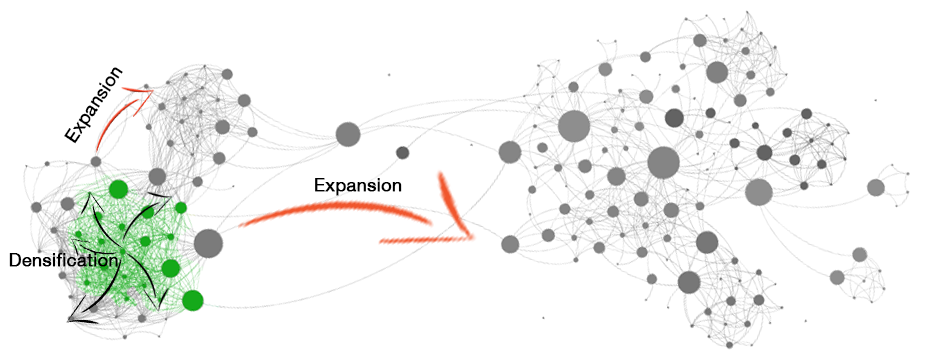
\includegraphics[width=0.5\textwidth]{concept}
    \caption{Concept of Expansion-Densification Algorithm}
    \label{fig:example}
\end{figure}

Algorithm \ref{exp-den} starts by collecting a small sample. The initial sample can be collected by any crawling technique. In our case, we adopt BFS crawling as shown in line 2.  BFS begins from any node $n_{start}$, queries the API for the node's neighbors, and adds all neighbors that have not been queried to an $\textit{unqueried}$ queue. The first node in the queue will be a next selected node. BFS is repeated for $budget_{bfs}$ times. All the nodes and edges found are kept as the initial sample. We define two types of nodes, $\textit{closed}$ and $\textit{open}$ node. A
$\textit{closed node}$ is a node that has already been queried. An $\textit{open node}$ is a node that has been observed, but not queried.

The main loop (line 3-7) of the algorithm switches between $Expansion$ and $Densification$, and it runs until it reaches a specified amount of budget. The input for $Expansion$ is the sample graph that obtained so far, and it returns a single node ($n_{exp}$), with the hope that $n_{exp}$ leads to a new region. $Densification$ acquires $n_{exp}$ as its input and tries to explore this new area of the network. It returns the sub-sample graph($S_{s}$). Finally, $S_{s}$ is merged with $S$.





\begin{algorithm}
\small
\caption{Exp-Den ({$budget, budget_{bfs}, n_{start}$})}\label{exp-den}
\begin{algorithmic}[1]
%\Function{Exp-den}{$budget, budget_{bfs}, n_{start}$}
\State $cost \gets 0$
\State $S \gets bfs(budget_{bfs}, n_{start})$ 
\While  {$cost \leq budget$}
	\State $n_{exp} \gets Expansion(S)$
	\State $S_{s} \gets Densification(n_{exp})$
	\State $S \gets $ Merge $S_{s}$ with $S$
\EndWhile
\end{algorithmic}
\end{algorithm}

\begin{center}
	\captionof{table}{Description of each variable} \label{tab:notation} 
    \begin{tabular}{  l | l }
    \hline
	 &  Description \\ \hline
	$N_{q}$ & a set of nodes returned from the API request\\
	$E_{q}$ & a set of edges returned from the API request\\
	$S$ & a sample graph $S(V',E')$ \\
	$S^{o}$ & a set of open nodes $n \in V'$\\
	$S^{c}$ & a set of closed nodes $n \in V'$\\
	$S_{s}$ & a sub-sample graph $S_{s}(V_{s},E_{s})$\\
	$S_{s}^{o}$ & a set of open nodes $n \in V_{s}$\\
	$S_{s}^{c}$ & a set of closed nodes $n \in V_{s}$\\
	$e_{ij}^{'}$ & $e_{ij} \in E_{s},(i \in S_{s}^{c} \wedge j \in S_{s}^{o})\vee(i \in S_{s}^{o} \wedge j \in S_{s}^{c}) $ \\
	$sc_{exp}^{t}$ & an expansion score at $t^{th}$ iteration \\
	$sc_{den}^{t}$ & a densification score at $t^{th}$ iteration \\
	$n_{exp}$ & a selected node from Expansion phase \\
	$w_{1}, w_{2}$ & weight \\	
	%$n_{c_{i}}$ & a set of nodes in $i^{th}$ community \\
	%$d_{c_{i}}$ & a diameter of $i^{th}$ community\\
	$|\cdot|$ & a cardinality of a set \\ \hline
    \end{tabular}
    
\end{center}


\begin{algorithm}
\caption{Densification ({$n_{cur}$})}\label{mod}
\begin{algorithmic}[1]
%\Function{MOD}{$n_{cur}$}
\State $S_{s} \gets empty$, $sc^{0}_{den} \gets 1$, $sc^{0}_{exp} \gets 0$
%\State $sc^{0}_{den} \gets 1$, $sc^{0}_{exp} \gets 0$
%\State $sc^{0}_{exp} \gets 0$\Comment{Set Expansion score to 0 }
\While {$sc^{t}_{exp} < sc^{t}_{den}$ or $cost < budget$}
	\State $N_{q}, E_{q} \gets $Make a query on $n_{cur}$
	
	\State $sc^{t}_{den} \gets w_{1}\times \frac{ \vert n \in N_{q} \backslash (S^{o} \cup S_{s}^{o} ) \vert }{\vert S_{s}^{c} \vert} + w_{2} \times sc^{t-1}_{den}$
	
%e(i,j) \in S_{s}^{e},(i \in S_{s}^{c} \wedge j \in S_{s}^{o})\vee(i \in S_{s}^{o} \wedge j \in S_{s}^{c}) 	
	
	\State $sc^{t}_{exp} \gets w_{1} \times  \frac{\vert e^{'}_{ij} \vert }{\vert S_{s}^{o} \vert}  + w_{2} \times sc^{t-1}_{exp}$
	\State $S_{s} \gets $ Add $N_{q}, E_{q}$ to sub sample
	\State $n_{cur} \gets $node with the highest degree in $S_{s}$
	\State $cost \gets cost + 1 $
\EndWhile

\Return $S_{s}$
%\EndFunction
\end{algorithmic}
\end{algorithm}

%\begin{algorithm}
%\caption{Expansion ({$S$})}\label{oracle}
%\begin{algorithmic}[1]
%	\For {$c_i $  in $C$}
%		\State $score_{i} \gets \frac{\vert n_{c_i} \vert}{|V|} \times  \frac{1}{d_{c_i}}$  \Comment{ score = gain x spread}
%	\EndFor
%	\State $ C_{target} = argmax(score_{i})$
%	
%	\For {$n $  in $S^{o}$}
%		\State $d_{n} \gets $ shortest path length from $n$ to $C_{target}$
%	\EndFor	
%	\State $ n_{best} = argmin(d_{n})$
%
%\Return $n_{best}$
%\end{algorithmic}
%\end{algorithm}



\textbf{Densification: }
To expand a sample within a region, we adopt Maximum Observed Degree (MOD)\cite{avrachenkov2014pay}, as it outperforms other algorithms in the same class. Pseudocode is shown in Algorithm \ref{mod}. In each iteration, the node with maximum degree is selected from $S_{s}^{o}$ and the algorithm requests its neighbors through the API. Nodes ($N_{q}$) and edges($E_{q}$) are returned and added to sub-sample ($S_{s}$). 

\textbf{Expansion: } In the Expansion step, the algorithm tries to escape from the current region of the network. The algorithm selects a node that will lead to another dense area. In the spirit of explore-exploit algorithms, one naive appoarch is to pick a node uniformly at random from $S^{o}$.  We refer this Expansion strategy as ``$random$" (in our future work, we examine other strategies for Expansion). 

\textbf{Switching Phases:}
Two scores are calculated in each iteration of Densification. Intuitively, in each step, the number of closed nodes increases while a number of new nodes added decreases over time (diminishing marginal returns). The algorithm will find many nodes in the same community at the beginning and this amount drastically drops when most of them are found. $sc^{t}_{den}$ measures how many new nodes are added to the sample after a request, divided by the number of closed nodes.  $sc^{t}_{exp}$ is the fraction of the number of edges ($e_{ij}^{'}$) connecting a closed node to an open node, divided by the number of open nodes in sub-sample.  If the number of edges $(e'_{ij})$ increases, the number of open nodes also increases. If not, it means the algorithm already found most of the nodes.  These scores give us an approximation of number of nodes left unexplored. Densification switches to Expansion when $sc^{t}_{exp}$ is higher than $sc^t_{den}$. Thus, the algorithm can appropiately switch between phases. 

%\textbf{Expansion: } In the Expansion step, we want to escape from the current part of the network. The algorithm selects a node in order to explore on another dense area. One naive appoarch is to pick one node uniformly at random from $S^{o}$, we refer this Expansion strategy as "$random$". Moreover, we introduce another appoarch, we refer as "$\textit{Oracle}"$. We assume that Oracle has the information of the entire graph. The pseudocode is shown in Algorithm \ref{oracle}. Firstly, Oracle selected a target community($C_{t}$) by considering the score (line 1-3). A community with the highest score is selected. The score is a multiplication of $gain$ and $spread$. $Gain$ measures a number of nodes left unexplored. $Spread$ measures how fast we can reach all the nodes in the community. We define spread is inversely proportional to the diameter of community($d_{c_{i}}$). After target community is selected, Oracle calculates the shortest path length from every open nodes($S^{o}$) to the target community. A node with the smallest distance is selected. Note that, we can improve the performance here by calculating clustering coefficient of all nodes in $S^{o}$ and ignore all node that the clustering coeffocient is equal to one. It is likely that these nodes are in the same community since the neighbors are tightly connected.

\section{Experiments and Discussion}

To mimic the process of querying an API, we simulate sampling from an existing network dataset. We compare our algorithm with the MOD algorithm\cite{avrachenkov2014pay}. For simplicity, we assume all networks are undirected. We use four different datasets, described in Table \ref{tab:dataset}. $\textit{Grad}$ and $\textit{Undergrad}$ are the Facebook networks \cite{mislove2010you}. $\textit{Enron-Email}$ is an email communication network. $Twitter$ is a friend-follower network that we collected via Twitter API.

\begin{table}
\centering
 %\captionof{table}{Names and statistics of datasets used in our work.} \label{tab:dataset} 
 	\caption{Names and statistics of datasets used in our work.}
 	\label{tab:dataset} 
    \begin{tabular}{ l | c | c | c | c }
    \hline
	 Network & \# Nodes & \# Edges & Global CC. & Mod. \\ \hline
	 Grad & 503 & 3256 & 0.4792 & 0.6915 \\
	 Undergrad & 1220 & 43208 & 0.2980 & 0.3937 \\
	 Twitter & 12230 & 50884 & 0.1117 & 0.6371 \\
	 Enron-Email & 36692 & 183831 & 0.4970 & 0.5975 \\ \hline
    \end{tabular}
   
\end{table}

\begin{figure}[h]
 	\centering
    \begin{subfigure}[t]{0.25\textwidth}
        \centering
        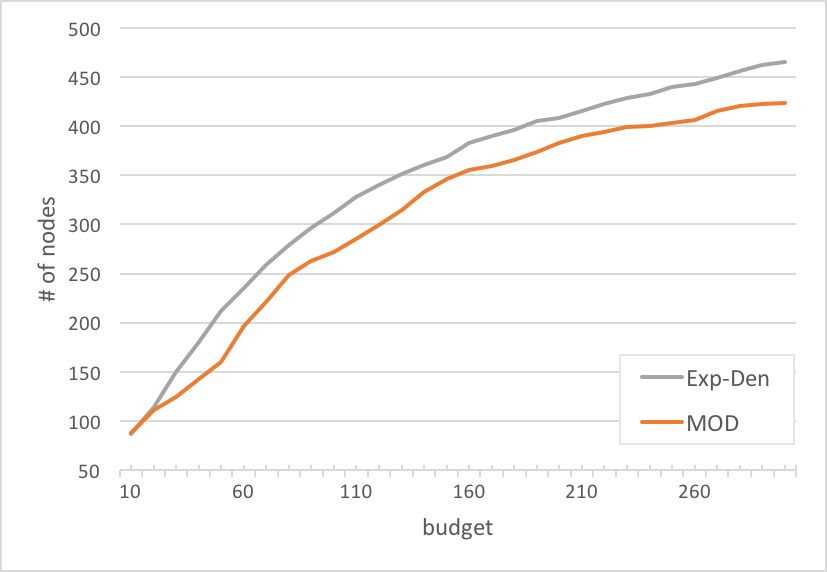
\includegraphics[height=1.1in]{grad2}
        \caption{Grad}
    \end{subfigure}%
    ~ 
    \begin{subfigure}[t]{0.25\textwidth}
        \centering
        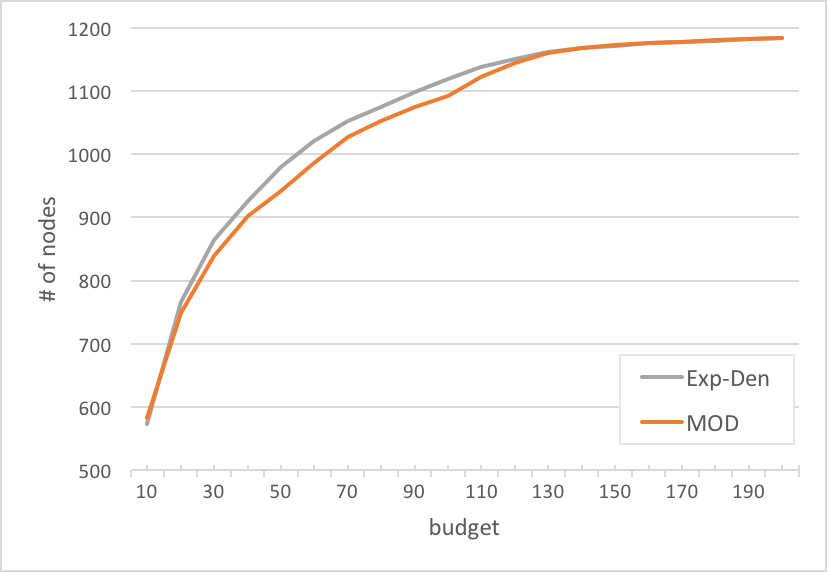
\includegraphics[height=1.1in]{undergrad2}
        \caption{Undergrad}
    \end{subfigure}
     \begin{subfigure}[t]{0.25\textwidth}
        \centering
        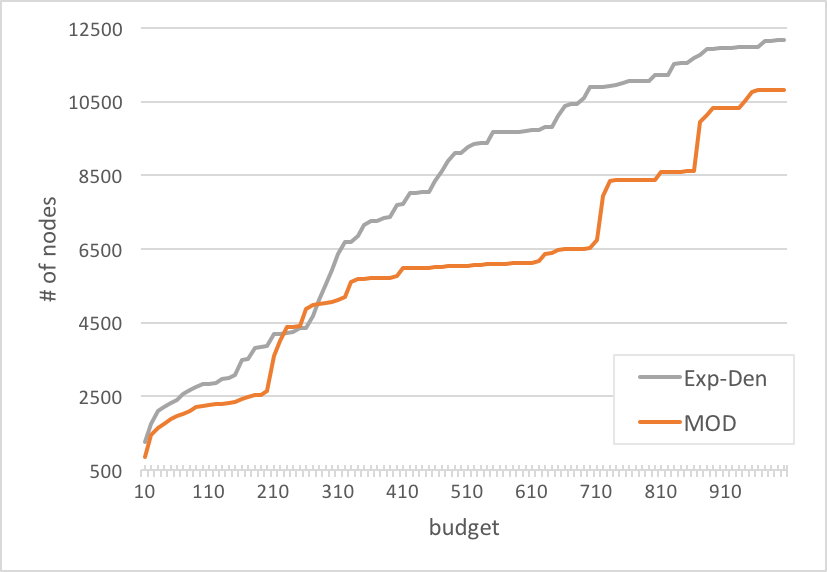
\includegraphics[height=1.1in]{twitter2}
        \caption{Twitter}
    \end{subfigure}%
    ~ 
    \begin{subfigure}[t]{0.25\textwidth}
        \centering
        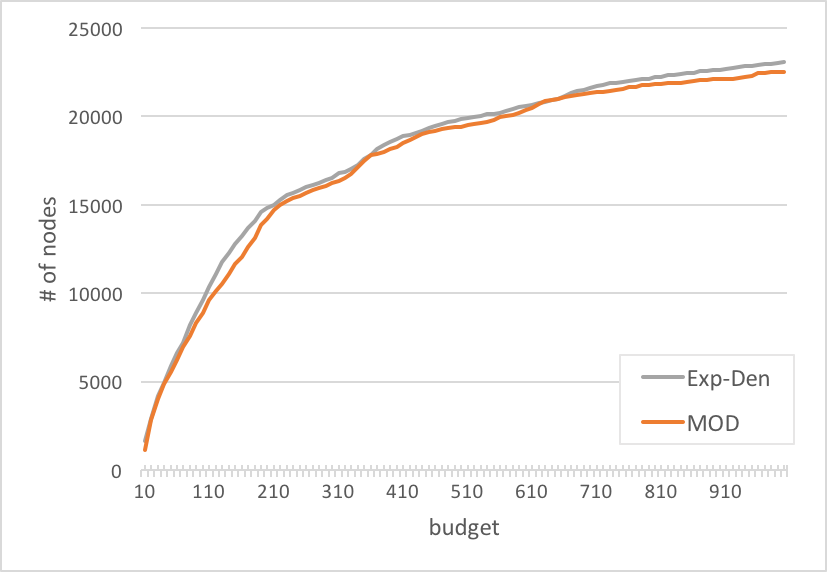
\includegraphics[height=1.1in]{enron2}
        \caption{Enron-Email}
    \end{subfigure}
   	 \caption{Experimental results on each dataset}\label{fig:result}
\end{figure}

We ran 15 experiments on each dataset, and plotted average values in Figure \ref{fig:result}. These plots depict the between amount of budget used versus the number of nodes obtained. Our algorithm outperformed MOD in every case. This gives us strong evidence that \ref{algo-name} algorithm is able to collect more nodes than MOD at the same amount of budget.  Interestingly, on the Twitter dataset, we clearly see that MOD becomes trapped in a region before being forced into a new region (indicated by steps in the result curve). A large budget is spent, but few nodes are added to the sample.

With a budget constraint, \ref{algo-name} performs well. Our future work includes improving the Expansion strategy with different switching criteria. 

%A criteria for switching between Densification and Expansion needs more studies.

\bibliographystyle{IEEEtran}
\bibliography{refs.bib}

% that's all folks
\end{document}


